\section{弱形式}
\label{sec:ellip-weak}

前面的公式都假设解有连续的二阶导数。这个假设常常不成立。考虑一根由两种材料接成的棒：$a=1$于$(0,1/2)$，$a=4$于$(1/2,1)$，源项$f=1$，两端温度为零。系数在中点跳变，方程~\eqref{eq:ellip-1d-equation}中的$(au')'$在中点该怎么理解？

\paragraph{一个没有经典解的问题}
先按物理来算。热流$q=-au'$满足$q'=1$，所以$q(x)=x+C$在整段上是一条直线；热流穿过界面时不会凭空消失，因而$q$连续。由此得到$u'=-(x+C)/a$，它在中点有跳跃。

再用$u(0)=u(1)=0$定常数。温度沿整段的变化为零：
\[
 0=\int_0^1u'\,\mathrm{d}x=-\int_0^{1/2}(x+C)\,\mathrm{d}x-\frac14\int_{1/2}^1(x+C)\,\mathrm{d}x .
\]

算出两个积分并代入，得到
\[
 -\Bigl(\frac18+\frac C2\Bigr)-\frac14\Bigl(\frac38+\frac C2\Bigr)=-\frac7{32}-\frac{5C}8=0,
\]
所以$C=-7/20$。中点的温度是$u(1/2)=-(1/8+C/2)=1/20=0.05$。

图~\ref{fig:ellip-coefficient-jump}是这个解。$u$连续而在中点有折角，$u'$从$-0.15$跳到$-0.0375$，所以$u$不是$C^2$函数，甚至不是$C^1$函数，在中点逐点谈论方程是没有意义的。可是物理上这个解完全合理，热流$q$也是连续的。我们需要一种能接纳它的“解”的定义。

\begin{BookInlineFigure}
  \centering
  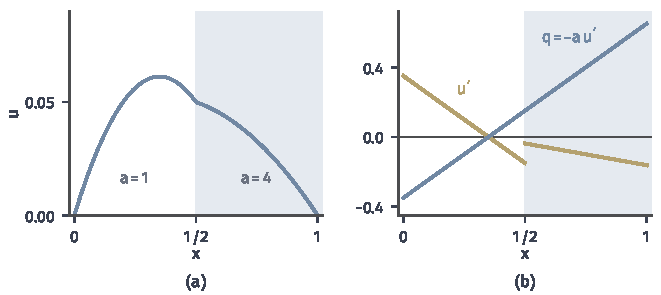
\includegraphics[width=112mm]{figures/06-differential-equations/02-partial-differential-equations/matplotlib/ellip-coefficient-jump/figure.pdf}
  \caption{两段材料接成的棒，$f=1$，两端温度为零，右半段（浅蓝底）导热率为$4$。(a)温度$u$连续，在中点有折角。(b)$u'$（黄）在中点跳跃，热流$q=-au'$（蓝）是一条连续的直线。}
  \label{fig:ellip-coefficient-jump}
\end{BookInlineFigure}

\paragraph{用测试函数检验}
经典解要求方程在每一点成立。换一种检验方式：取光滑的“探针”函数$v$，它只在某一小块区域内不为零，读取方程两边在这块区域上的加权平均。若对所有探针读数都相等，就说方程成立。这样的$v$称为\term{测试函数}（test function）。

用式~\eqref{eq:ellip-1d-equation}检验：两边乘以在两端为零的$v$，积分，并分部积分一次，把一个导数从$au'$移到$v$上：
\[
 \int_0^1fv\,\mathrm{d}x=-\int_0^1(au')'v\,\mathrm{d}x=\int_0^1au'v'\,\mathrm{d}x-\bigl[au'v\bigr]_0^1 .
\]
$v$在两端为零，边界项消失，于是
\begin{equation}
 \int_0^1a\,u'v'\,\mathrm{d}x=\int_0^1fv\,\mathrm{d}x .
 \label{eq:ellip-weak-1d}
\end{equation}

式~\eqref{eq:ellip-weak-1d}只含$u$的一阶导数，$a$也不需要可导。上面的折线型解可以直接代入。取$v=x(1-x)$，$v'=1-2x$，由$au'=-(x+C)$，两段合起来得到
\[
 \int_0^1au'v'\,\mathrm{d}x=-\int_0^1\Bigl(x-\frac7{20}\Bigr)(1-2x)\,\mathrm{d}x=\frac16,
\]
右端$\int_0^1fv\,\mathrm{d}x$也是$\int_0^1x(1-x)\,\mathrm{d}x=1/6$，两边相等。界面处的通量连续性不用单独写，它已经包含在弱形式中。

\begin{BookInlineFigure}
  \centering
  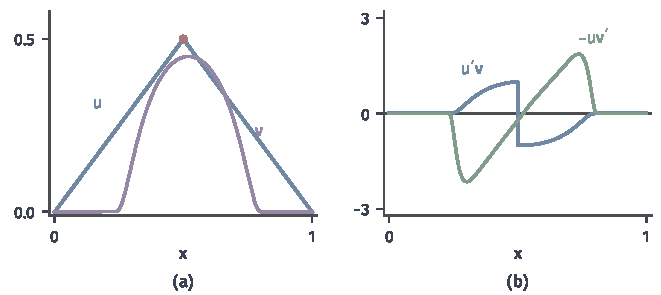
\includegraphics[width=112mm]{figures/06-differential-equations/02-partial-differential-equations/matplotlib/ellip-test-probe/figure.pdf}
  \caption{把导数转移到测试函数上。(a)$u=\tfrac12-\lvert x-\tfrac12\rvert$在红点处有折角，紫线是支撑在$(0.22,0.82)$内的光滑测试函数$v$（画为$0.45$倍）。(b)蓝线$u'v$在折角处跳跃，绿线$-uv'$连续。两条曲线不同，下方的积分却相同，数值积分都约为$-0.040$。}
  \label{fig:ellip-test-probe}
\end{BookInlineFigure}

这个动作的实质是让测试函数承担一半的导数，如图~\ref{fig:ellip-test-probe}所示。卷四用同样的动作定义了弱导数，这里只是把它用于方程。下面把多维的对应写出来，$\bm{A}$的条件沿用定义~\ref{def:ellip-uniform}。

\paragraph{多维的分部积分}
设$\Omega$是有界Lipschitz区域，$u,v$足够光滑。向量场$v\,\bm{A}\nabla u$的散度由乘积法则给出：
\[
 \nabla\cdot(v\bm{A}\nabla u)=\nabla v\cdot\bm{A}\nabla u+v\,\nabla\cdot(\bm{A}\nabla u) .
\]
对它用散度定理，得到
\begin{equation}
 \int_\Omega\bigl(-\nabla\cdot(\bm{A}\nabla u)\bigr)v\,\mathrm{d}\bm{x}
 =\int_\Omega\bm{A}\nabla u\cdot\nabla v\,\mathrm{d}\bm{x}-\int_{\partial\Omega}(\bm{n}\cdot\bm{A}\nabla u)\,v\,\mathrm{d}S .
 \label{eq:ellip-green-first}
\end{equation}
这是Green第一恒等式的一般形式。左端要两阶导数，右端的体积分只要一阶，边界项显示了边界通量在哪里出现。

由此定义贯穿全章的\term{双线性型}（bilinear form）
\begin{equation}
 a(u,v)=\int_\Omega\bm{A}\nabla u\cdot\nabla v\,\mathrm{d}\bm{x}.
 \label{eq:ellip-bilinear}
\end{equation}

\paragraph{用到的空间}
式~\eqref{eq:ellip-bilinear}有意义，只需要$u,v$有平方可积的一阶弱导数，这就是Sobolev空间$H^1(\Omega)$。回忆几个事实，其详细讨论可参考\BookChapterRef{chap:sobolev-spaces}{卷四第21章“Sobolev空间”}：

\begin{itemize}
 \item $H^1(\Omega)$由$L^2(\Omega)$中弱梯度也在$L^2$中的函数组成，按函数值和梯度的$L^2$内积之和定义内积后，它是Hilbert空间；
 \item 在有界Lipschitz区域上，存在把$H^1(\Omega)$映到$L^2(\partial\Omega)$的有界线性迹算子$\operatorname{Tr}$，对光滑到边界的函数就是限制到边界；
 \item $H^1_0(\Omega)$是$C_c^\infty(\Omega)$在$H^1$范数下的闭包，有界Lipschitz区域上它恰好是迹为零的函数组成的闭子空间。
\end{itemize}

本章记$\lVert v\rVert_2$为$L^2(\Omega)$范数，$\lVert\nabla v\rVert_2$为$\lVert\nabla v(\bm{x})\rVert_2$的$L^2(\Omega)$范数，$H^1$范数则由下式给出：
\[
 \lVert v\rVert_{H^1}^2=\lVert v\rVert_2^2+\lVert\nabla v\rVert_2^2 .
\]

函数值在边界上的约束要借助迹来表达，因为$H^1$函数只是几乎处处定义的等价类，边界是零测集，不能读取一个代表的边界值。右端的$\int_\Omega fv$只要求$f\in L^2(\Omega)$，甚至可以更弱：只要$v\mapsto\ell(v)$是$H^1_0(\Omega)$上的有界线性泛函。这样的泛函全体记为$H^{-1}(\Omega)$。

下面按边界条件的类型分别写出弱形式。两类条件的处理方式完全不同：一类写进函数空间，一类写进积分。

\subsection{Dirichlet条件}
\label{sec:ellip-weak-dirichlet}

对问题$-\nabla\cdot(\bm{A}\nabla u)=f$，$u=g$于$\partial\Omega$，式~\eqref{eq:ellip-green-first}中含未知的边界通量。测试函数取零迹时，这一项直接消失，所以测试函数应取在$H^1_0(\Omega)$中。

解要满足边界值$g$，这是对$u$的约束，写成$\operatorname{Tr}u=g$。要让这个条件有意义，$g$必须是某个$H^1(\Omega)$函数的迹，满足这个要求的边界函数组成迹空间，通常记为$H^{1/2}(\partial\Omega)$。于是有下面的定义。

\begin{definition}[Dirichlet问题的弱解]
\label{def:ellip-weak-dirichlet}
设$\Omega$是有界Lipschitz区域，$\bm{A}$一致椭圆，$f\in L^2(\Omega)$，$g=\operatorname{Tr}R$，其中$R\in H^1(\Omega)$。若$u\in H^1(\Omega)$满足$\operatorname{Tr}u=g$，且
\begin{equation}
 a(u,v)=\int_\Omega fv\,\mathrm{d}\bm{x}\qquad\text{对所有}\ v\in H^1_0(\Omega),
 \label{eq:ellip-weak-dirichlet}
\end{equation}
就称$u$是该问题的\term{弱解}（weak solution）。式~\eqref{eq:ellip-weak-dirichlet}称为\term{弱形式}（weak formulation）。
\end{definition}

这里要分清两组函数。候选的解称为试探函数，它们组成的集合是$\{u\in H^1(\Omega):\operatorname{Tr}u=g\}$，$g\neq0$时这不是线性空间，两个解之和的迹是$2g$。测试函数在$H^1_0(\Omega)$中，它是线性空间。

\paragraph{边界提升}
两者的关系是：试探函数的集合是$H^1_0(\Omega)$的一个平移。取任一满足$\operatorname{Tr}R=g$的函数$R$，称为$g$的\term{边界提升}（boundary lifting），令$w=u-R$，则$w\in H^1_0(\Omega)$。代入式~\eqref{eq:ellip-weak-dirichlet}，由$a$的双线性，问题化为
\begin{equation}
 a(w,v)=\int_\Omega fv\,\mathrm{d}\bm{x}-a(R,v)\qquad\text{对所有}\ v\in H^1_0(\Omega).
 \label{eq:ellip-lifted}
\end{equation}
边界数据的影响进入了右端的泛函，$w$在线性空间$H^1_0(\Omega)$中寻找，见图~\ref{fig:ellip-affine-trial}。

\begin{BookInlineFigure}
  \centering
  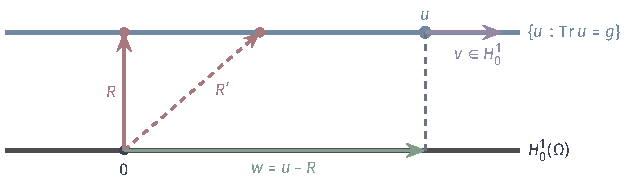
\includegraphics[width=110mm]{figures/06-differential-equations/02-partial-differential-equations/tikz/ellip-affine-trial/figure.pdf}
  \caption{试探集合与测试空间。深灰线是线性空间$H^1_0(\Omega)$，蓝线是平行的试探集合$\{u:\operatorname{Tr}u=g\}$，红色箭头是两个不同的提升$R$与$R'$。解$u$落在蓝线上，$w=u-R$（绿）在$H^1_0(\Omega)$中；试探集合内的移动方向（紫）都属于$H^1_0(\Omega)$，这就是测试函数取自$H^1_0(\Omega)$的原因。}
  \label{fig:ellip-affine-trial}
\end{BookInlineFigure}

提升不唯一，但$u$与提升的选择无关。回到例子$-u''=1$，$u(0)=1$，$u(1)=3$，解是$1+2x+x(1-x)/2$。取$R=1+2x$，得$w=x(1-x)/2$；取$R'=1+2x^2$，得$w'=5x(1-x)/2$。两个$w$不同，$R+w$与$R'+w'$却是同一个函数。

\paragraph{经典解与弱解}
新定义是否与原问题一致？经典解一定是弱解，反过来，足够光滑的弱解也是经典解，下面的定理说明了这一点。

\begin{theorem}[经典解与弱解]
\label{thm:ellip-classical-weak}
设$\Omega$是有界Lipschitz区域，$\bm{A}\in C^1(\overline\Omega)$一致椭圆，$f\in C(\overline\Omega)$，$u\in C^2(\overline\Omega)$，且在$\partial\Omega$上$u=g$。则$u$是弱解当且仅当
\begin{equation}
 -\nabla\cdot(\bm{A}\nabla u)=f\qquad\text{在}\ \Omega\ \text{内逐点成立}.
 \label{eq:ellip-classical}
\end{equation}
\end{theorem}

\begin{proof}
设$u$逐点满足方程。两边乘以$v\in C_c^\infty(\Omega)$，用式~\eqref{eq:ellip-green-first}，边界项为零，得到$a(u,v)=\int fv$。两边对$v$在$H^1$范数下都连续，$C_c^\infty(\Omega)$在$H^1_0(\Omega)$中稠密，所以等式对所有$v\in H^1_0(\Omega)$成立。

反过来，设$u$是弱解。对$v\in C_c^\infty(\Omega)$，式~\eqref{eq:ellip-weak-dirichlet}与式~\eqref{eq:ellip-green-first}合起来给出
\[
 \int_\Omega\bigl(-\nabla\cdot(\bm{A}\nabla u)-f\bigr)v\,\mathrm{d}\bm{x}=0 .
\]
括号内的函数连续。若它在某点不为零，就在该点附近保持同号，取在那里为正的局部凸起$v$，积分不为零，矛盾。所以它处处为零。
\end{proof}

用一个例子看弱形式怎样接纳更粗糙的数据。在$(0,1)$上固定$y$，令$\ell(v)=v(y)$，这是点源。$H^1_0(0,1)$的函数有连续代表，由Cauchy--Schwarz不等式，
\[
 \lvert v(y)\rvert=\Bigl\lvert\int_0^yv'\,\mathrm{d}x\Bigr\rvert\leq\sqrt y\,\lVert v'\rVert_2 ,
\]
所以$\ell$是有界泛函。Green函数$G(\cdot,y)$的斜率在$y$的左右分别是$1-y$和$-y$，代入弱形式，
\[
 \int_0^1G_x\,v'\,\mathrm{d}x=(1-y)\bigl(v(y)-v(0)\bigr)-y\bigl(v(1)-v(y)\bigr)=v(y),
\]
可见帐篷函数就是点源问题的弱解。

一维的这个例子不能推广到高维。$d\geq2$时$H^1$函数不必连续，点值不是有界泛函，点源的解$\Phi$的梯度也不平方可积，这一点在第~\ref{sec:ellip-lax-milgram}小节还会用到。

\subsection{Neumann与Robin条件}
\label{sec:ellip-weak-neumann}

若边界上规定的是通量，式~\eqref{eq:ellip-green-first}的边界项恰好是已知的量，这时不必再让它消失。

\paragraph{Neumann问题}
设$\bm{n}\cdot\bm{A}\nabla u=g$于$\partial\Omega$，$g\in L^2(\partial\Omega)$。两边乘以$v\in H^1(\Omega)$，用式~\eqref{eq:ellip-green-first}，把边界通量换成$g$，移到右端：
\begin{equation}
 a(u,v)=\int_\Omega fv\,\mathrm{d}\bm{x}+\int_{\partial\Omega}gv\,\mathrm{d}S\qquad\text{对所有}\ v\in H^1(\Omega),
 \label{eq:ellip-weak-neumann}
\end{equation}
其中边界积分里的$v$是迹。这里的试探函数和测试函数都在整个$H^1(\Omega)$中，空间没有施加任何边界约束。

\paragraph{Robin问题}
设$\bm{n}\cdot\bm{A}\nabla u+\beta u=g$，$\beta\geq0$。边界通量写成$g-\beta u$，代入后含未知函数$u$的边界项移到左端，得到
\begin{equation}
 a_\beta(u,v)=\int_\Omega fv\,\mathrm{d}\bm{x}+\int_{\partial\Omega}gv\,\mathrm{d}S\qquad\text{对所有}\ v\in H^1(\Omega),
 \label{eq:ellip-weak-robin}
\end{equation}
其中双线性型多了一个边界项：
\begin{equation}
 a_\beta(u,v)=a(u,v)+\int_{\partial\Omega}\beta uv\,\mathrm{d}S.
 \label{eq:ellip-robin-bilinear}
\end{equation}

\paragraph{边界条件怎样从积分中回来}
式~\eqref{eq:ellip-weak-neumann}没有明写边界条件，它是怎样被满足的？设弱解足够光滑。先取$v\in C_c^\infty(\Omega)$，边界项都消失，由定理~\ref{thm:ellip-classical-weak}的论证得到内部方程。

把内部方程代回，对一般的$v\in H^1(\Omega)$，式~\eqref{eq:ellip-green-first}给出
\[
 \int_{\partial\Omega}(\bm{n}\cdot\bm{A}\nabla u-g)\,v\,\mathrm{d}S=0 .
\]
$v$的边界值可以任意变动，所以$\bm{n}\cdot\bm{A}\nabla u=g$成立。这样由弱形式自动产生的条件称为\term{自然边界条件}（natural boundary condition）。对比之下，Dirichlet条件要事先放进试探集合，称为\term{本质边界条件}（essential boundary condition）。

用混合问题看这个机制的效果。方程$-u''=1$，$u(0)=0$，$u'(1)=0$，真解是$u_*=x-x^2/2$。弱形式是：$u$满足$u(0)=0$，且对所有$v(0)=0$的$v\in H^1(0,1)$有$\int_0^1u'v'\,\mathrm{d}x=\int_0^1v\,\mathrm{d}x$。

假如取一个满足内部方程但边界条件错误的候选$\tilde u=x(1-x)/2$，定义残量
\[
 R(v)=\int_0^1\tilde u'v'\,\mathrm{d}x-\int_0^1v\,\mathrm{d}x .
\]
分部积分，因$-\tilde u''=1$，积分项消去，只剩边界项：
\[
 R(v)=\bigl[\tilde u'v\bigr]_0^1=\tilde u'(1)\,v(1)=-\frac{v(1)}2 .
\]

图~\ref{fig:ellip-natural-residual}(b)画出这个关系。只要测试函数在$x=1$处不为零，$\tilde u$就通不过检验，而$u_*$对所有测试函数残量为零。例如$v=x$时，$\tilde u'v'=\tfrac12-x$的积分为$0$，$\int_0^1v=\tfrac12$，所以$R(v)=-\tfrac12$，与公式相符。

\begin{BookInlineFigure}
  \centering
  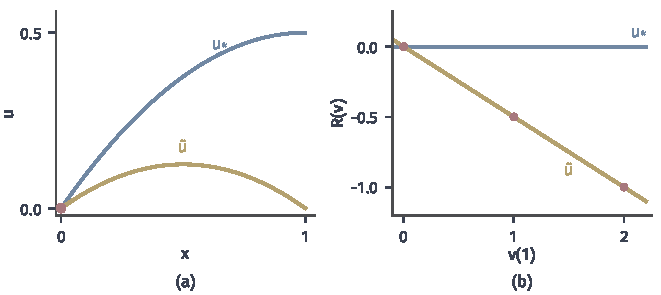
\includegraphics[width=112mm]{figures/06-differential-equations/02-partial-differential-equations/matplotlib/ellip-natural-residual/figure.pdf}
  \caption{自然边界条件由测试函数在边界上的自由度强制。(a)真解$u_*$（蓝）与错误候选$\tilde u$（黄），后者满足$u(1)=0$而不满足$u'(1)=0$。(b)残量$R(v)$随$v(1)$的变化，红点依次是$v=x(1-x)$、$v=x$或$x^2$、$v=2x$；$u_*$的残量恒为零。}
  \label{fig:ellip-natural-residual}
\end{BookInlineFigure}

把两类条件的对比列成表~\ref{tab:ellip-boundary-weak}。三种条件的差异只在于：边界的值由谁来负责。

\begin{BookInlineTable}
  \centering
  \caption{三类边界条件的弱形式。}
  \label{tab:ellip-boundary-weak}
  \begin{tabular}{llll}
    \toprule
    条件 & 试探函数 & 测试函数 & 边界数据的去向\\
    \midrule
    Dirichlet & $\operatorname{Tr}u=g$ & $H^1_0(\Omega)$ & 写进空间（本质）\\
    Neumann & $H^1(\Omega)$ & $H^1(\Omega)$ & 右端边界积分（自然）\\
    Robin & $H^1(\Omega)$ & $H^1(\Omega)$ & 左端$\beta$项与右端积分（自然）\\
    \bottomrule
  \end{tabular}
\end{BookInlineTable}
